\section{Additional Results in Model Wind Tunnel Experiments}

\subsection{$\mu$P hyper-parameter search}
\label{app:bayesiansearch}
Meanwhile, we also try QK-Norm~\citep{henry-etal-2020-query} and independent weight decay~\citep{loshchilov2017decoupled} as well to stabilize the learning rate. The overall results are shown in Figure~\ref{fig:mupsearch_app}. After applying the QK-norm, we observe a significant decrease in the learning rate sensitivity similar to~\cite{wortsman2023small}. In Figure~\ref{fig:mupsearch_app}, we identify the best hyper-parameters for $scale\_depth=1.4$, $scale\_emb=12$, $init\_std=0.1$, and $lr=0.01$. 

\begin{figure}[htbp]
    \centering
    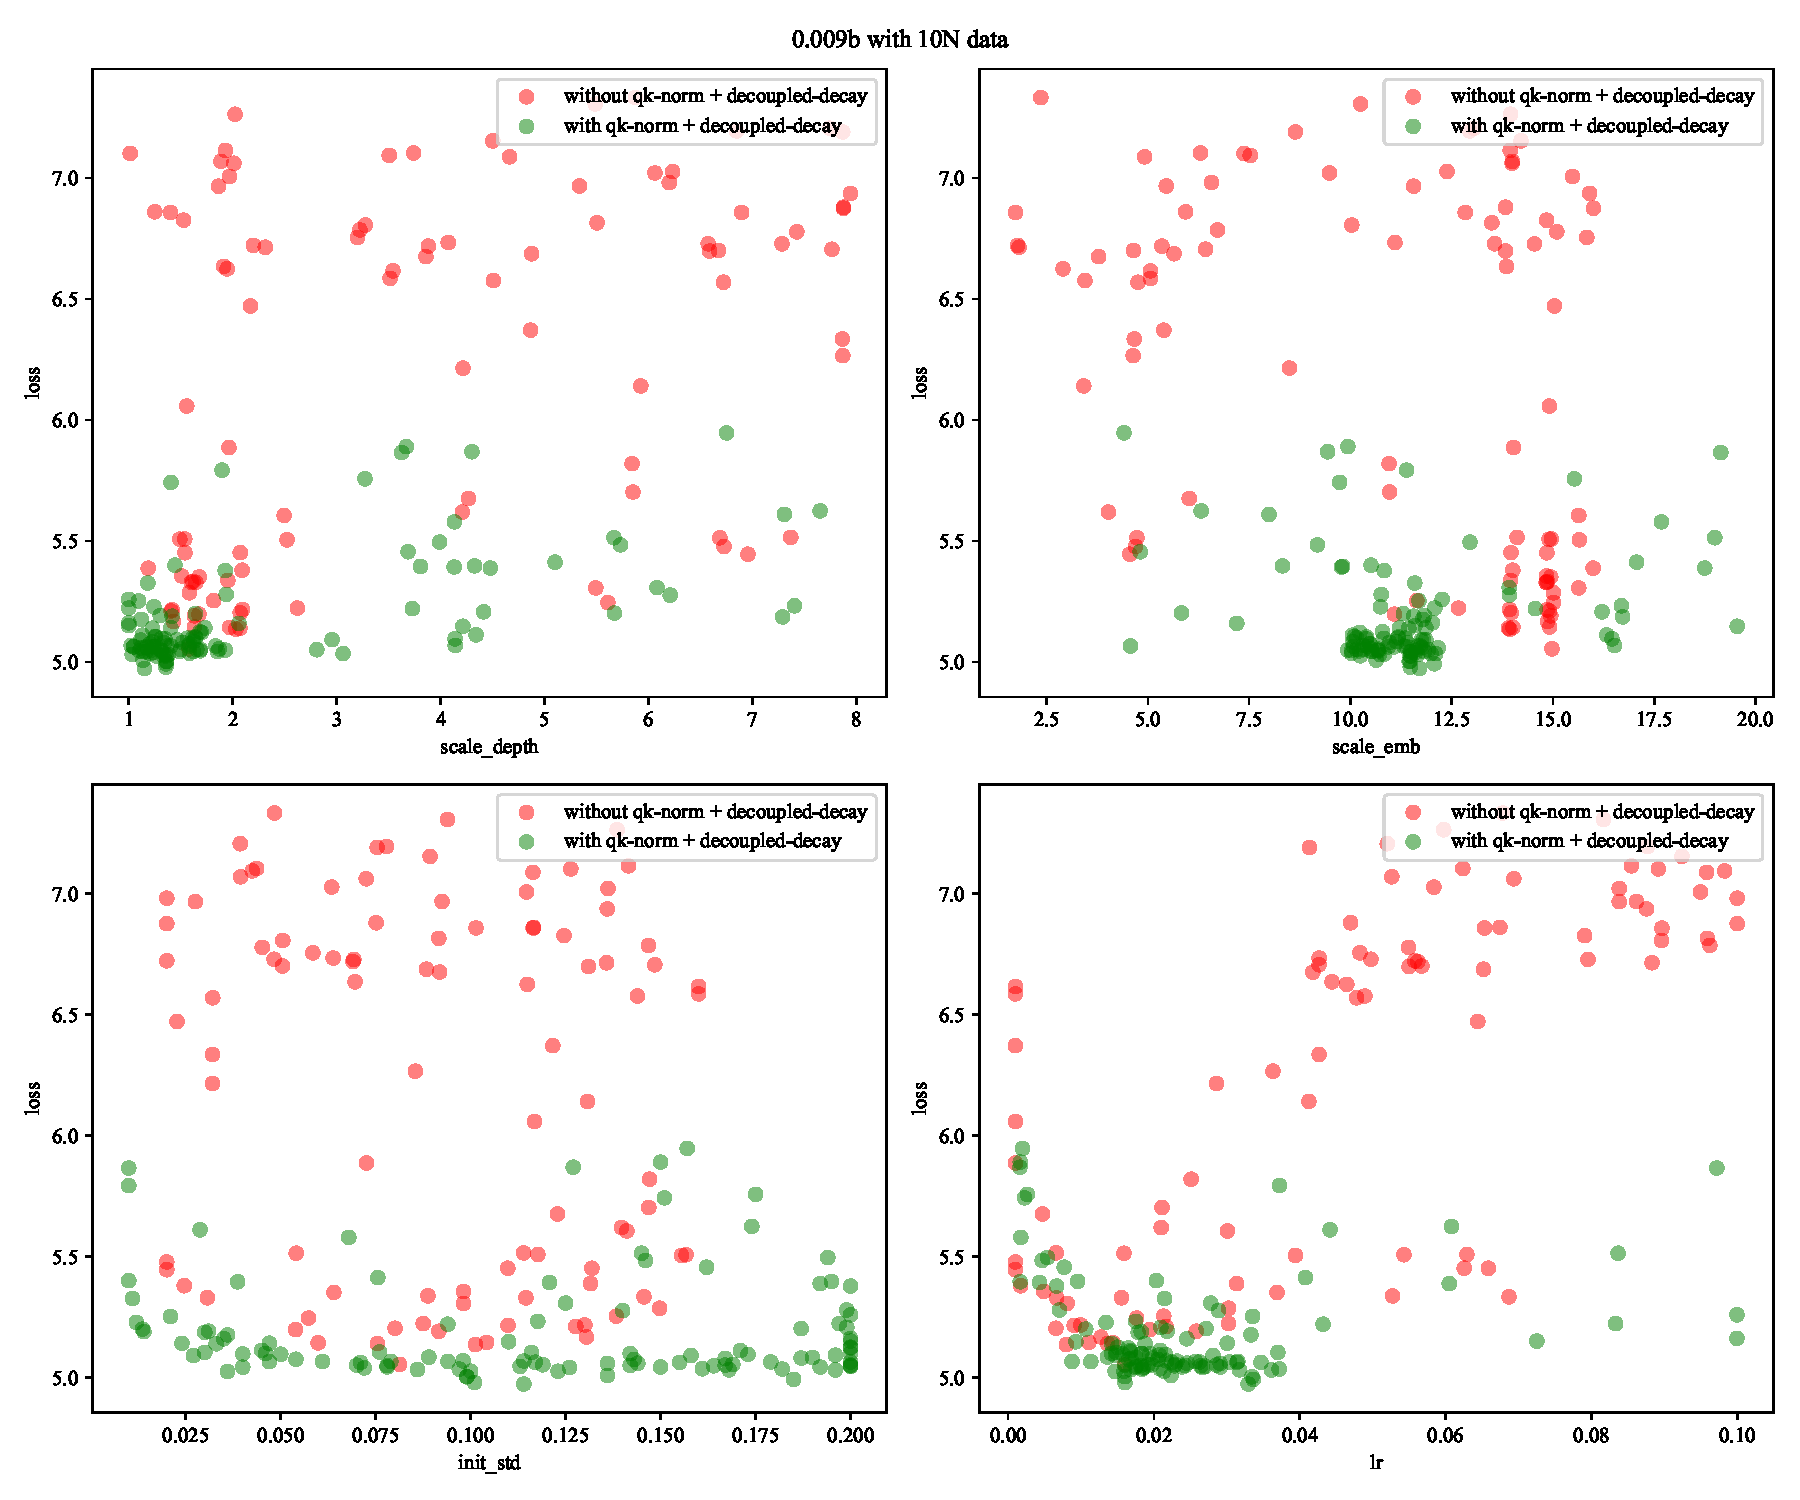
\includegraphics[width=0.65\linewidth]{Fig/mup0.009bwith10Ndata.pdf}
    \caption{Grid search over the $\mu$P parameterization spaces.}
    \label{fig:mupsearch_app}
\end{figure}

\begin{table}[h]
\centering
\begin{tabular}{l|p{8cm}}
\toprule
\textbf{Name}                       & \textbf{Specific Operation}                                                                                                                 \\ \midrule
Embedding Output Scaling            & Multiply the output of the embedding by $scale\_{emb}$                                                                                                                                                     \\ \hline
Residual Connection Scaling         & Scale the output tensor of a block before adding to each residual connection in each layer by $scale\_{depth}/\sqrt{\text{num\_layers}}$ 
\\ \hline
Initialization of Tensors           & Set the initialization standard deviation of each two-dimensional tensor parameter to $init\_std/\sqrt{d_m/d_{base}}$, and set other parameters' initialization to 0.1                  \\ \hline
Learning Rate Scaling of Tensors    & Adjust the learning rate of each two-dimensional tensor parameter to $1/({d_m/d_{base}}) $ times the learning rate of other parts (or the overall learning rate)                    \\ \hline
LM Head Scaling                    & Adjust the output logits to $1/(d_m/d_{base})$ times the original value                                                                                                           \\ \bottomrule
\end{tabular}
\caption{List of operations used when applying tensor program techniques.}
\label{tab:mup}
\end{table}

\subsection{Model Architecture in Model Wind Tunnel Experiments}
We list the model configuration used in the model wind tunnel experiments in Table~\ref{tab:appmodel_configs}.

\begin{table}[htbp]
    \centering
    \begin{tabular}{c|cccccc}
    \toprule
        \textbf{Name} & \textbf{N (B)}& $d_m$ & $d_{ff}$ &$d_h$ & $n_h$ & $L$ \\
    \midrule
          9M    &  0.009 & 320 & 800 & 64 & 5 & 8\\
           30M &   0.036 & 512 & 1280 & 64 & 8 & 12  \\
          70M &  0.066 & 640 & 1600 & 64 & 10 & 14\\
          0.1B &  0.109 & 768 & 1920 & 64 & 12 & 16  \\
         0.17B &  0.166 & 896 & 2240 & 64 & 14 & 18 \\
         0.2B&  0.241 & 1024 & 2560 & 64 & 16 & 20 \\
        0.5B& 0.499 & 1344 & 3360 & 64 & 21 & 24 \\
    \bottomrule
    \end{tabular}
    \caption{Model configurations and training configurations of the models in the scaling curve. N(B) represents the number of non-embedding parameters of the models, measured in billions.
    }
    \label{tab:appmodel_configs}
\end{table}

\section{Additional Illustration on WSD LRS}
\subsection{Learning Rate Paradigm for Different LRSs}
\label{app:lrsequ}
In this paper, we describe three kinds of LRSs, $Cosine(T)$, $CosineLoop(T)$, and $WSD(T, D)$. 
Cosine and Cosine Loop take the form of the following:

\begin{figure}[htbp]
    \centering
    % First minipage for the first figure
    \begin{minipage}{0.47\linewidth}
        \begin{equation*}
    \begin{aligned}
    & Cosine(T; s) = \\
    & \begin{cases}
       & \frac{s}{W} \eta, \quad s<W \\
       & 0.9\eta cos(\pi \frac{s}{T}) + 0.1\eta, \quad W < s < T \\
       & 0.1\eta,\quad  s > T \\
    \end{cases}
\end{aligned}
        \end{equation*}
    \end{minipage}
    \hfill % This adds a little space between the two figures
    % Second minipage for the second figure
    \begin{minipage}{0.52\linewidth}
             \begin{equation*}
    \begin{aligned}
    & CosineLoop(T; s) = \\
    & \begin{cases}
       & \frac{s}{W} \eta, \quad s<W \\
       & 0.9\eta cos(\pi \frac{s}{T}) + 0.1\eta, \quad W < s  \\
    \end{cases}
\end{aligned}
        \end{equation*}
    \end{minipage}
\end{figure}


An illustrative learning rate diagram for WSD and Cosine Scheduler is shown in Figure~\ref{fig:learning_rate_scheduler_diagram}.


\begin{figure}[!htbp]
    \centering
    \begin{minipage}{0.45\linewidth}
    % First minipage for the first figure
        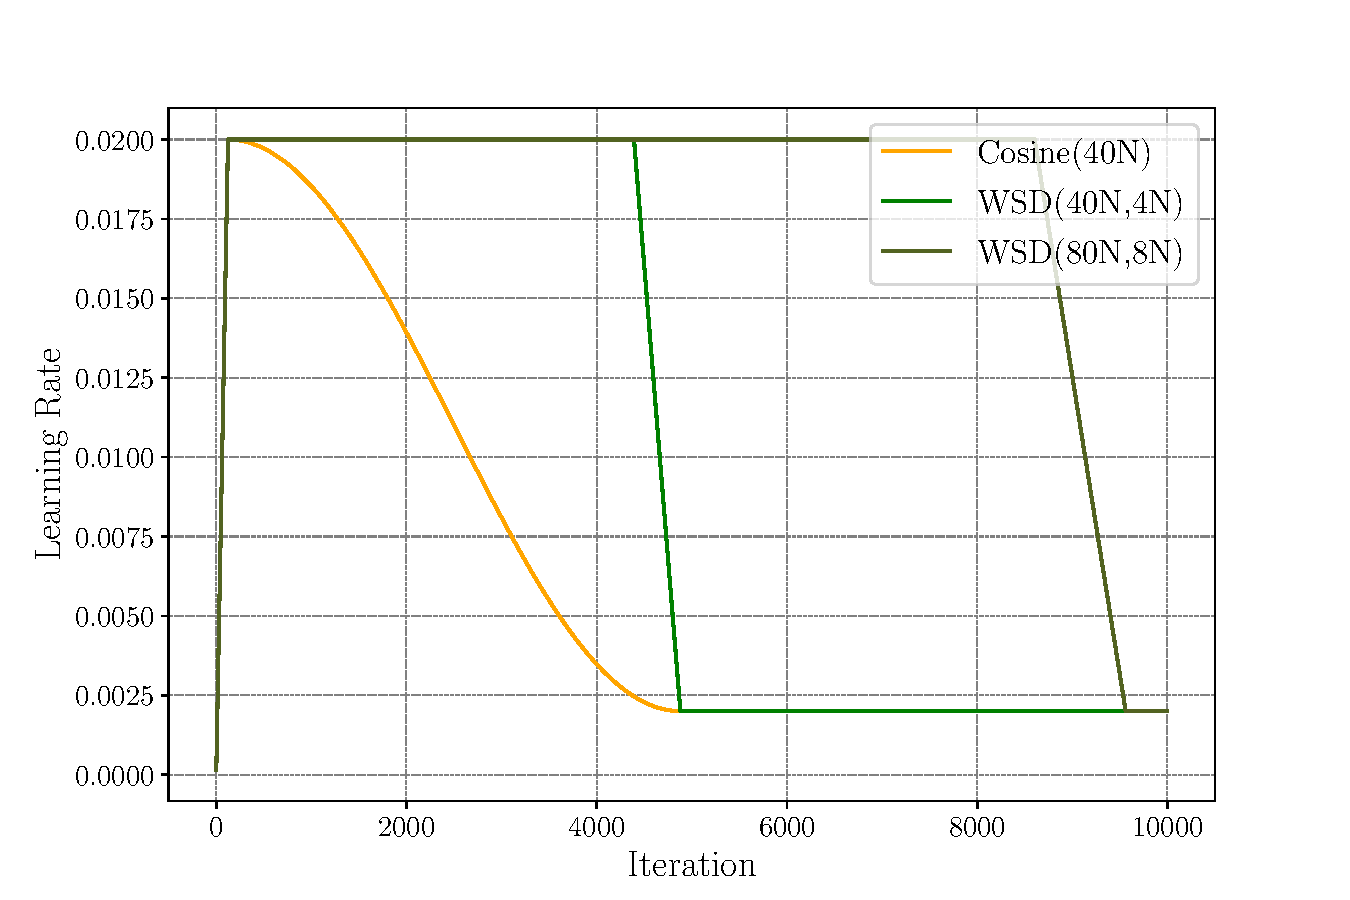
\includegraphics[width=0.98\linewidth]{Fig/lr.pdf}
        \caption{Illustrative comparison between Cosine LRS and WSD LRS. The WSD LRS with different end steps share the same stable training stage. }\label{fig:learning_rate_scheduler_diagram}
    \end{minipage}
        \begin{minipage}{0.45\linewidth}
    \centering
    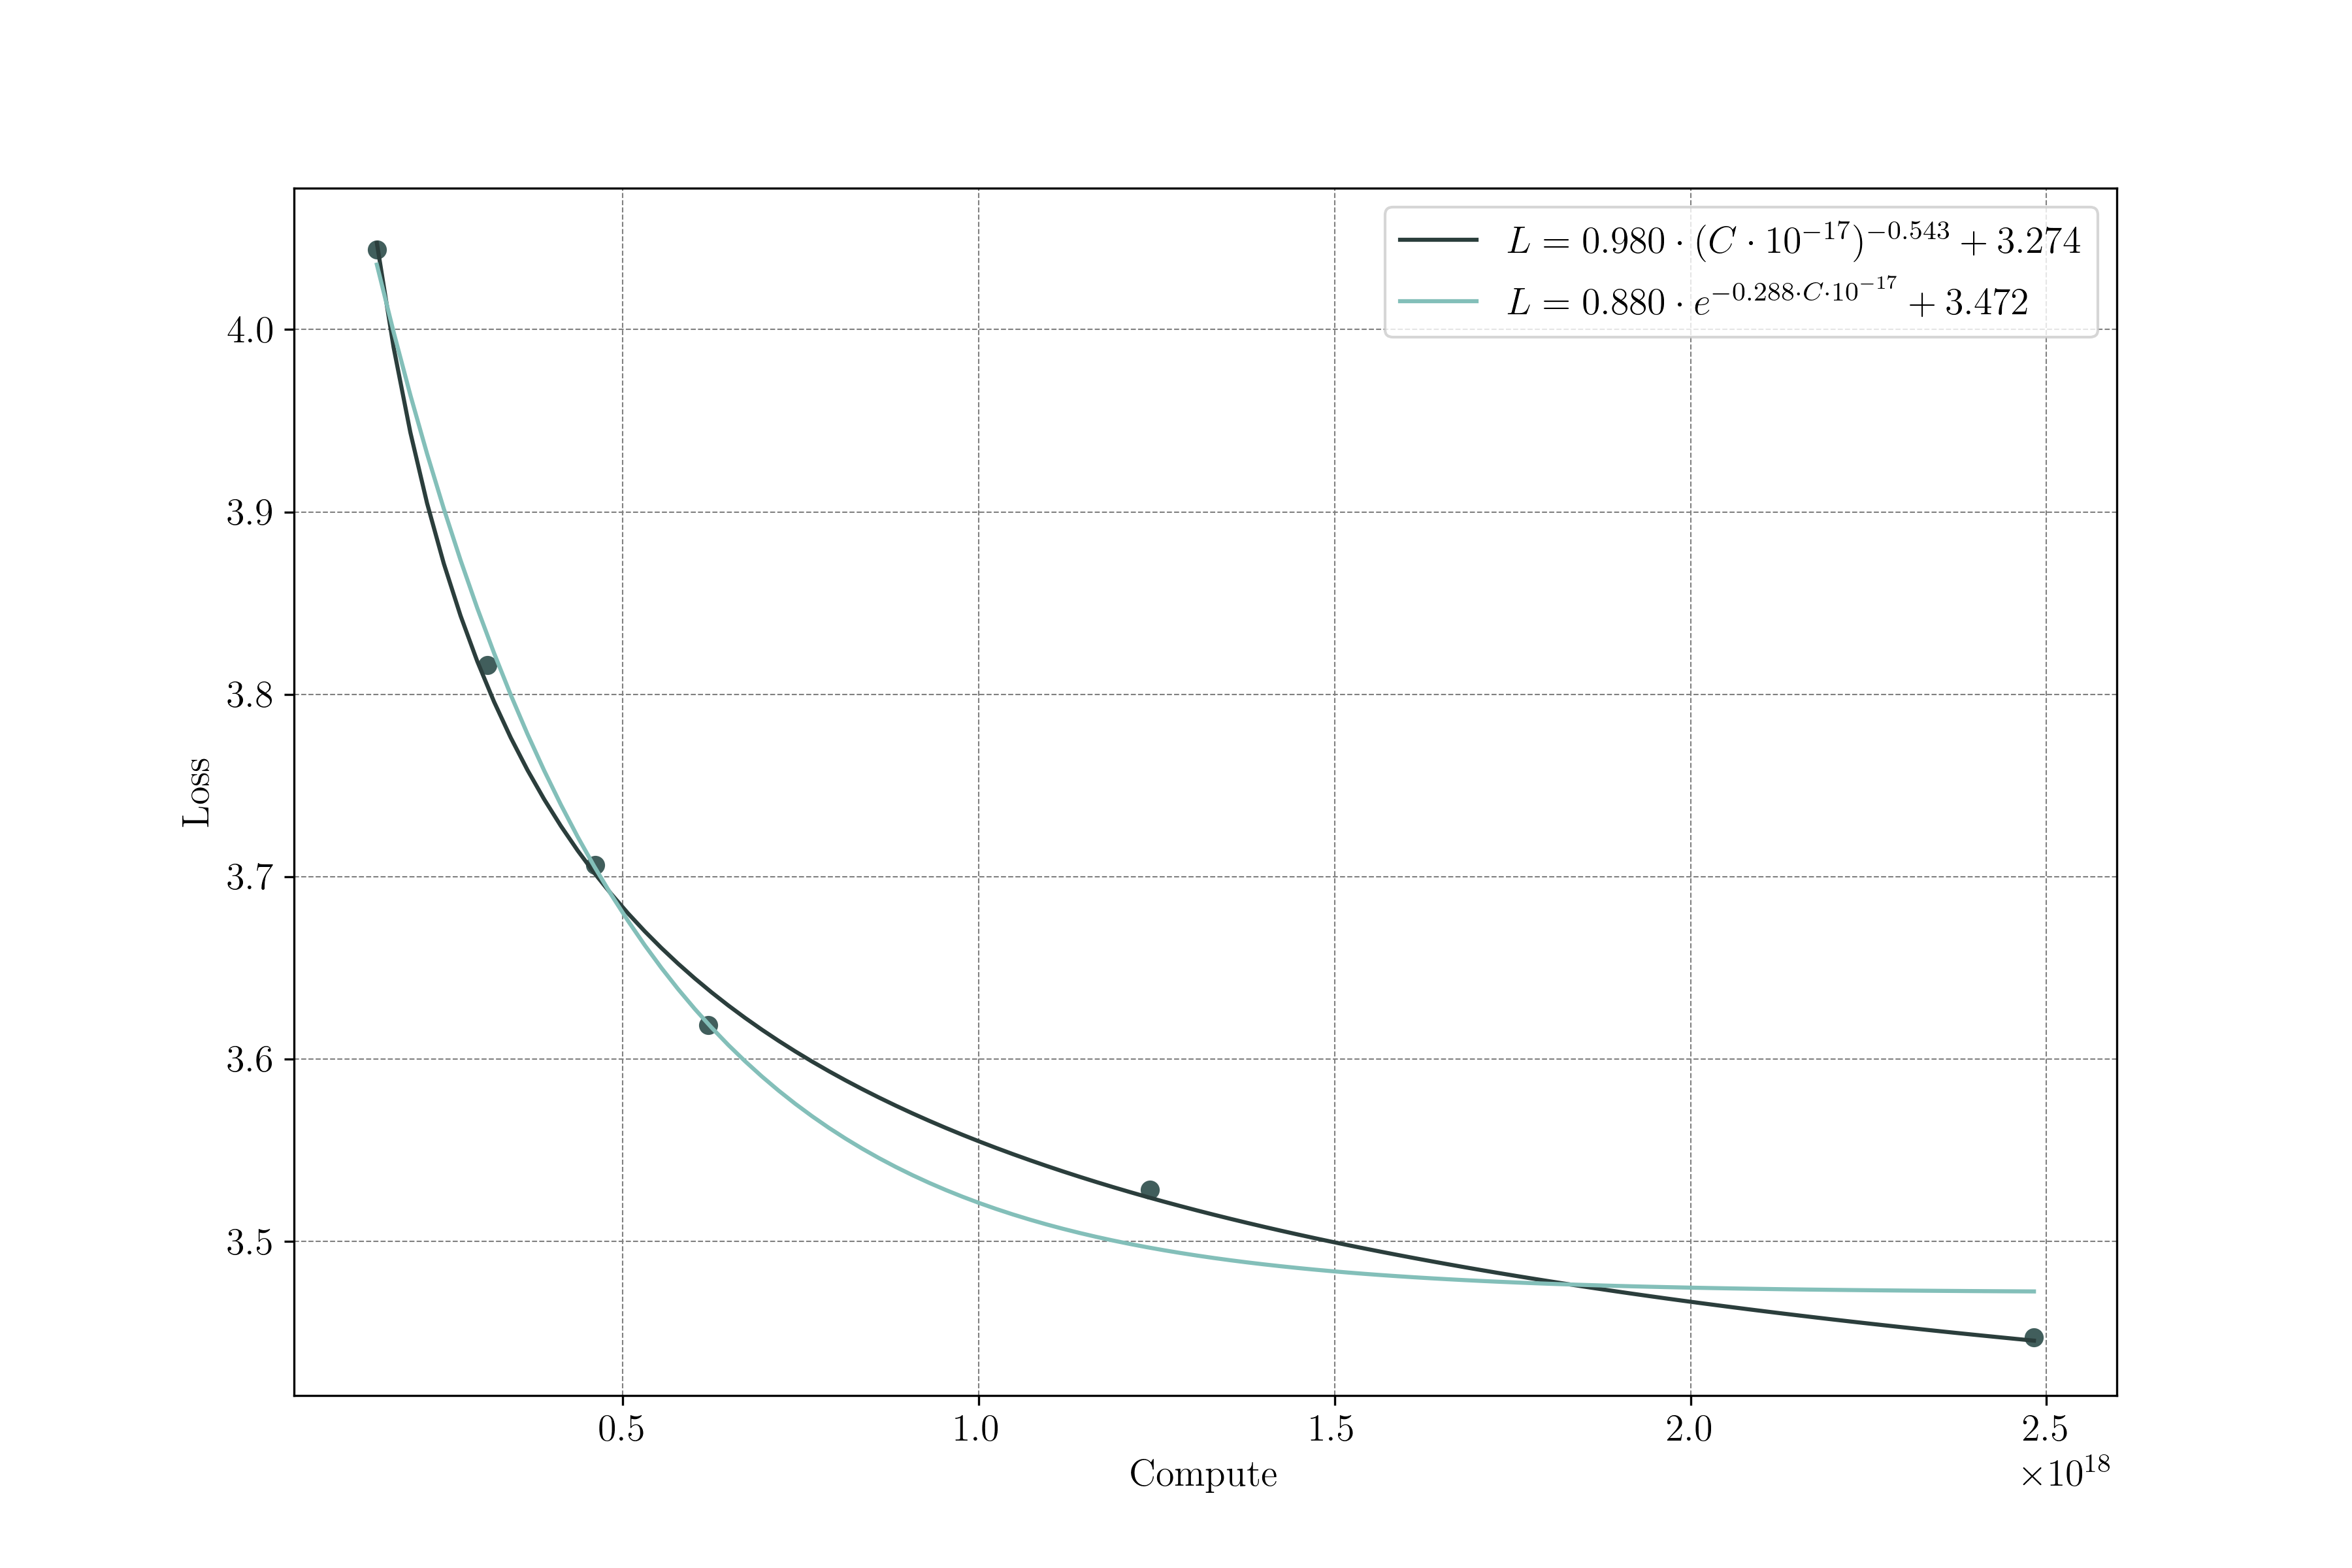
\includegraphics[width=1.05\linewidth]{Fig/fit_continuetrain.png}
    \caption{We use two different function forms to fit the data scaling law achieved by WSD LRS and choose power law as the best fit.}
    \label{fig:fit_continue_train}
    \end{minipage}
\end{figure}


\subsection{Fitting the Data Scaling Law}
\label{app:fittingdatascaling}
In this section, we describe the fitted data scaling law for continue training with WSD LRS. 
Each point in Figure~\ref{fig:fit_continue_train} is the end of the decay stage in WSD LRS with a different end step. We try two function forms: exponential and polynomial. The fitted result shows that the polynomial scaling law is still the best for continue training.

\subsection{Individual Figure for Model-Data Scaling Law}
For each task and model, the scaling law $L(N, D)$'s fitness with real loss values along the data axis is plotted in Figure~\ref{fig:individual_task_datascalinglaw}.

\begin{figure}
    \centering
    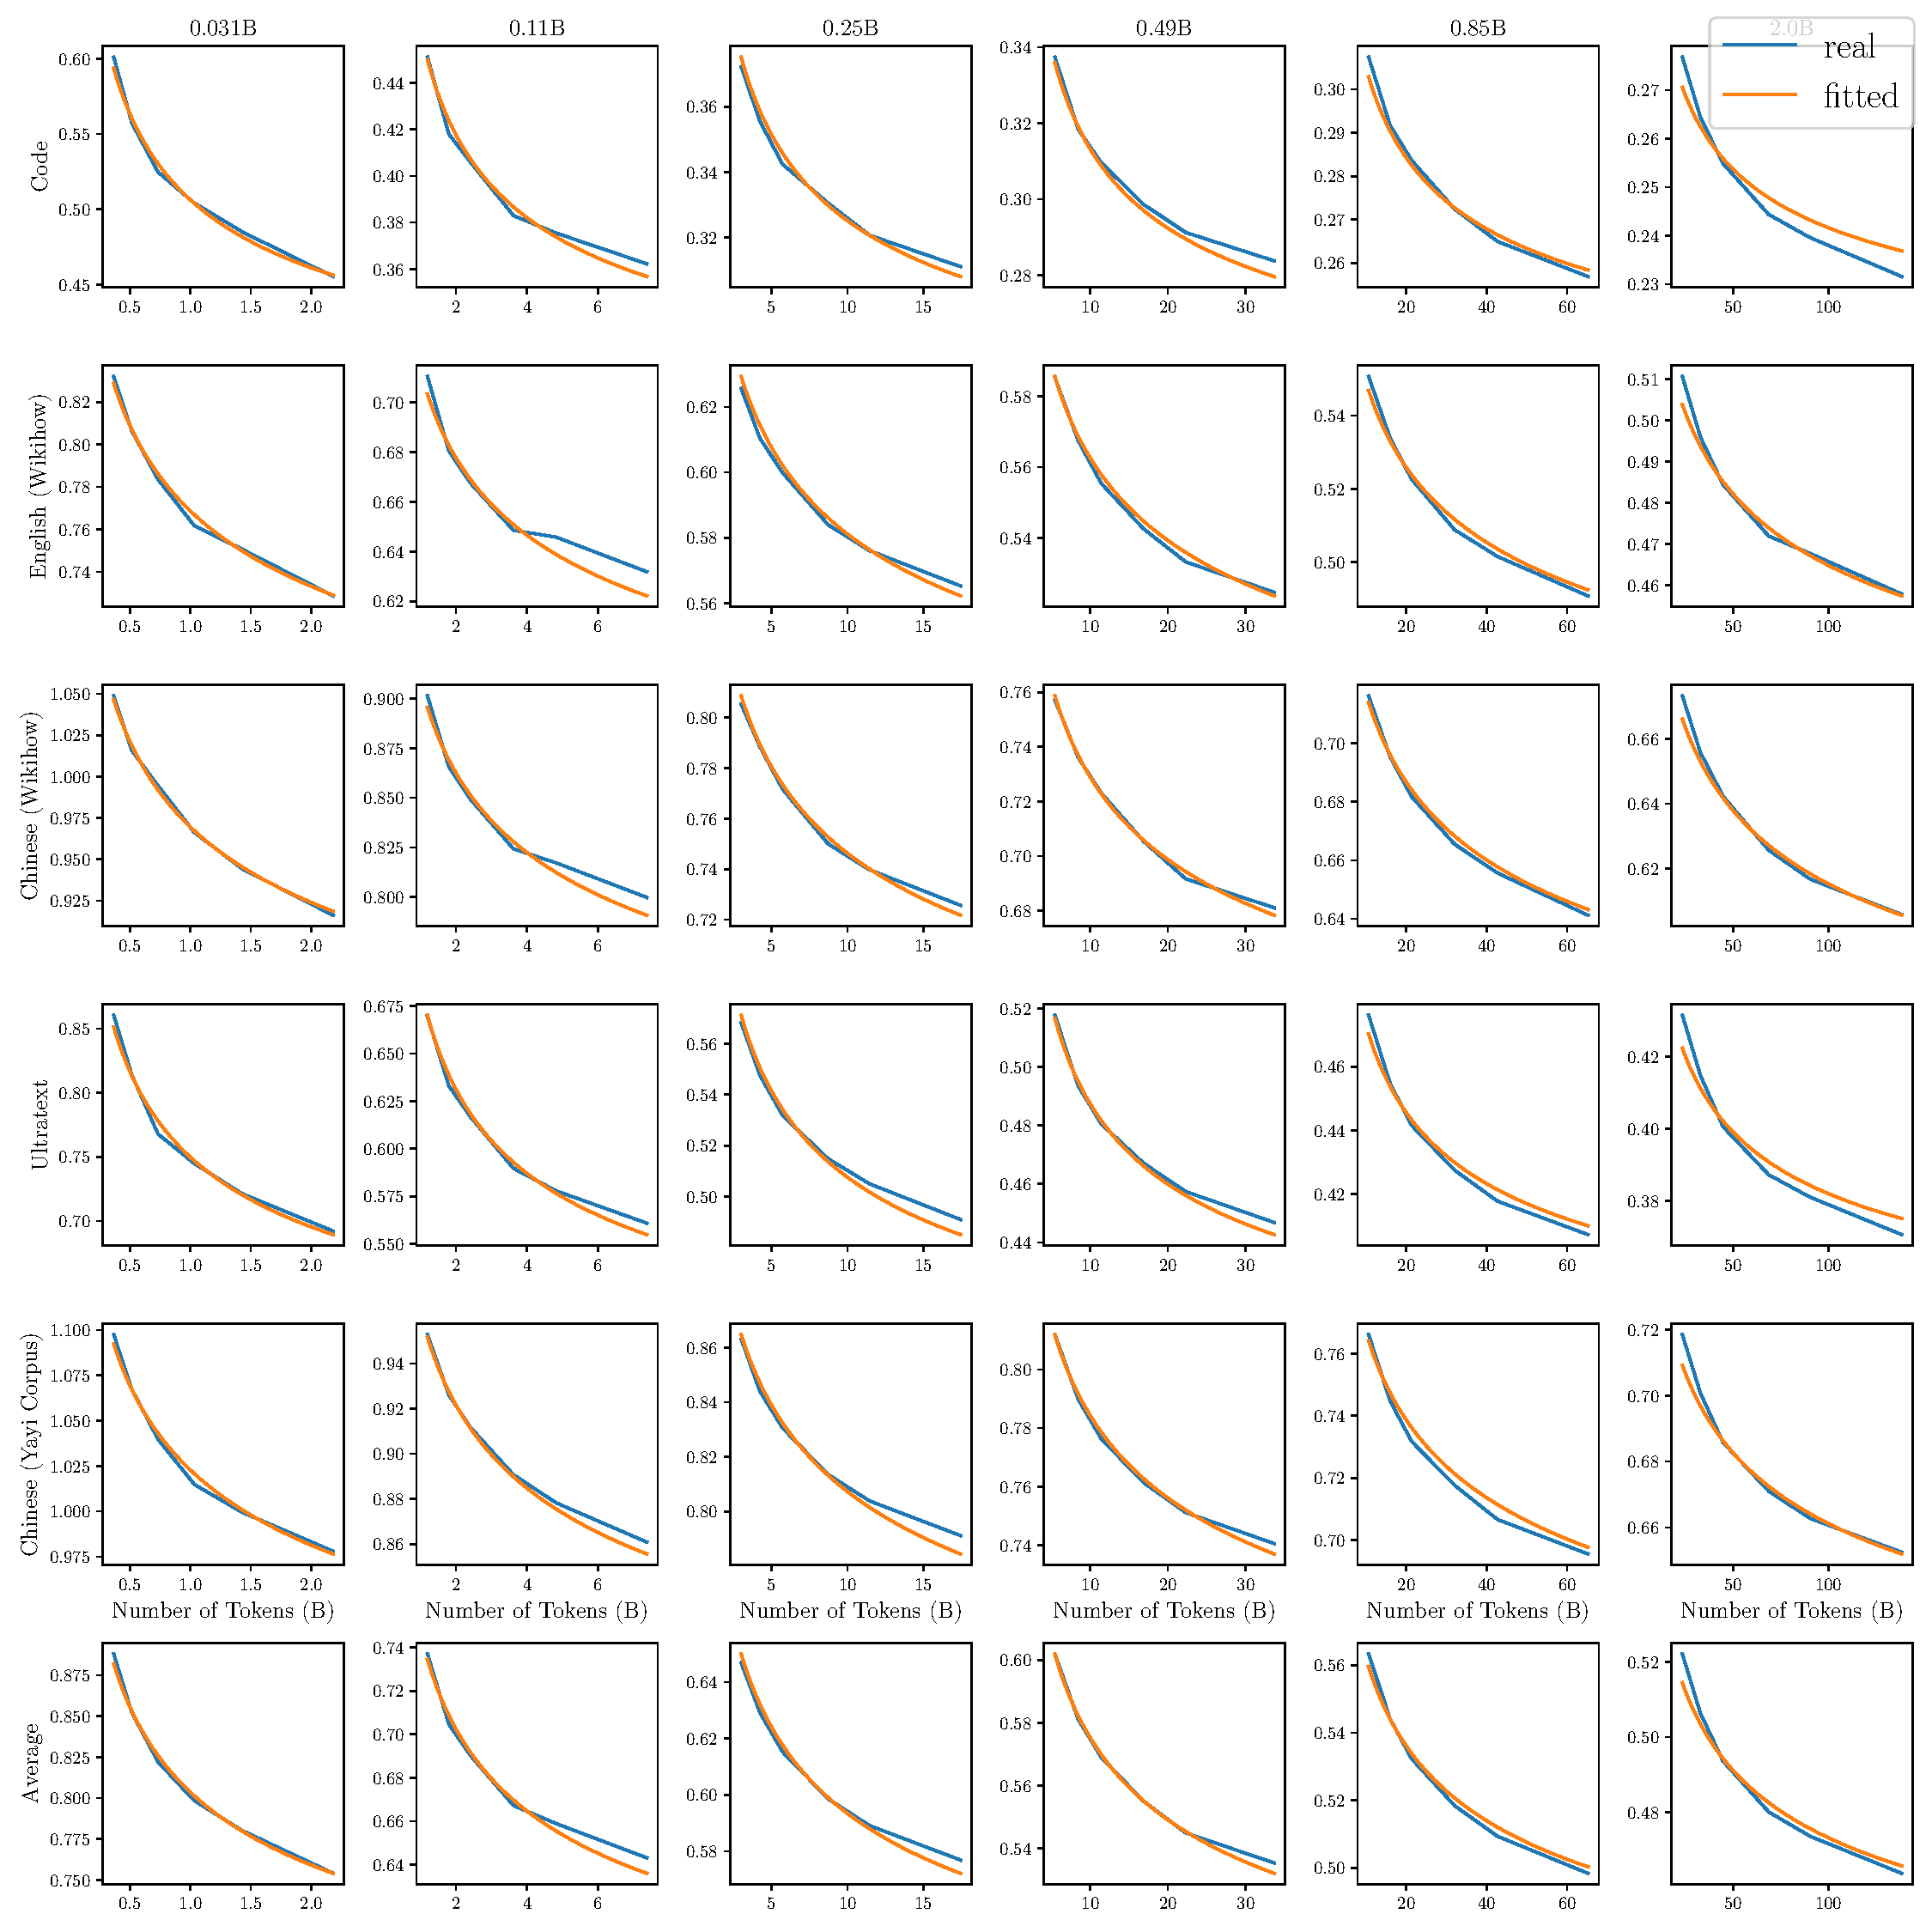
\includegraphics[width=1.0\textwidth]{Fig/individual_task_datascalinglaw.pdf}
    \caption{The fitted scaling law plotted along the data amount axis for each model and each task. The fitted result is satisfying except for the last checkpoints of the 0.11B and 0.25B model. }
    \label{fig:individual_task_datascalinglaw}
\end{figure}

\section{MiniCPM's Vocabulary}
\label{app:tokenizer}

For the 2.4B model, we use a tokenizer consisting of 122,753 tokens (denoted by MiniCPMTokenizer-120K). This vocabulary is constructed from extensive and diverse language data, utilizing the sentencepiece library~\footnote{\url{https://github.com/google/sentencepiece}} for Byte Pair Encoding (BPE)~\citep{sennrich-etal-2016-neural}, and includes special symbols like \uline{traditional Chinese characters}, \uline{rare characters}, \uline{emojis}, and special symbols such as \uline{Greek letters}, \uline{Cyrillic letters}, etc.

For our 1.2B model, we use a smaller vocab MiniCPMTokenizer-70K. Compared to the MiniCPMTokenizer-120K tokenizer, we have re-trained the tokenization on the same documents, while setting the max number of vocabs to \uline{64,000}. For the special characters, we only add the \uline{traditional Chinese characters}, \uline{emojis}, and \uline{special symbols}, but leave out the rare characters in Chinese. 

We conduct evaluations on 300,000 documents in Chinese, English, code, and academic papers that are not in the training set of the Tokenizer. \uline{The MiniCPM-120K tokenizer achieves the highest compression ratio (Bytes/Tokens).}

\begin{table}[htbp]
\centering
\begin{tabular}{lccccc}
\toprule
  & {\textbf{Baichuan2}}  & {\textbf{ChatGLM2}} & {\textbf{Llama2}} & {\textbf{MiniCPM-120K}}  & {\textbf{MiniCPM-70K}}\\
\midrule
Vocab Size & 125,696 & 64,794 & 32,000 & 122,753 & 73,440\\
\midrule
\multicolumn{6}{c}{\textbf{Compression Rate} (Bytes/Tokens) }\\
\midrule
Chinese & 3.64   & 3.54  & 1.87  & \textbf{3.73} &  3.56 \\
English & 4.12   & 4.02  & 3.78  & \textbf{4.14} & 4.02 \\
Code    & 2.71   & 2.71  & 2.74  & \textbf{2.81} & 2.76 \\
Paper   & 2.74   & 2.88  & \textbf{2.97}  & 2.93 & 2.88\\
\midrule
Average & 3.30   & 3.29  & 2.84  & \textbf{3.40}  & 3.31 \\
\bottomrule
\end{tabular}
\caption{Compression ratio comparison.}
\label{tab:compression_ratio}
\end{table}